\documentclass[../main.tex]{subfiles}
\usepackage{../style}
\graphicspath{ {../img/} }
\begin{document}
\chapter{RCL with AC}
\section{Alternating Current}
Direct current (DC) circuits involve current flowing in one direction. In alternating current (AC) circuits, instead of a constant voltage supplied by a battery, the voltage oscillates in a sine wave pattern, varying with time as $ V = V_0 \sin \omega t $.\\

In a household circuit, the frequency is $ 60 $ Hz. The angular frequency is related to the frequency, $ f $, by $ \omega = 2nfV_0 $ represents the maximum voltage, which in a household circuit in North America is about $ 170 $ volts. We talk of a household voltage of $ 120 $ volts, though; this number is a kind of average value of the voltage. The particular averaging method used is something called root-mean-square (square the voltage to make everything positive, find the average, take the square root), or rms. Voltages and currents for AC circuits are generally expressed as r.m.s. values. For a sine wave, the relationship between the peak and the r.m.s. average is:
\[\text{r.m.s. value} =0.707 \text{ peak value}\]
\begin{figure}[ht]
    \centering
    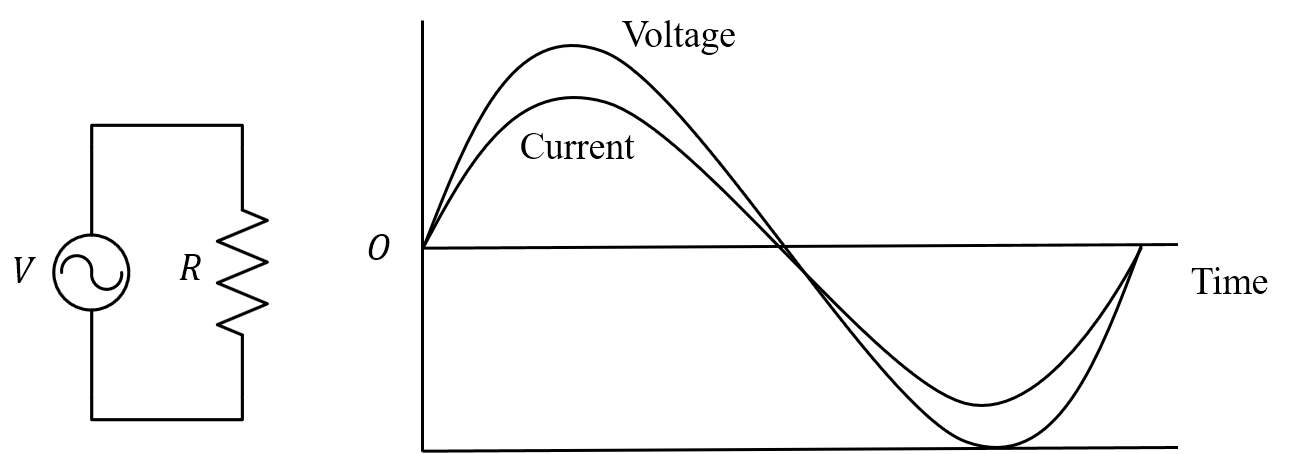
\includegraphics[scale=.75]{ac-circuit-1.png}
\end{figure}
% The relationship $ V=IR $ applies for resistors in an AC circuit, so 
% \[
%     I=\frac{V}{R}=\frac{V_0}{R}\sin(\omega t)=I_0\sin(\omega t)
% \]
\section{Resistance in an AC circuit}
The relationship $ V=IR $ applies for resistors in an AC circuit, so 
\[
    I=\frac{V}{R}=\frac{V_0}{R}\sin(\omega t)=I_0\sin(\omega t)
\]

In AC circuits we'll talk a lot about the phase of the current relative to the voltage. In a circuit which only involves resistors, the current and voltage are in phase with each other, which means that the peak voltage is reached at the same instant as peak current. In circuits which have capacitors and inductors (coils) the phase relationships will be quite different.
\section{Capacitance in an AC circuit}
\begin{figure}[ht]
    \centering
    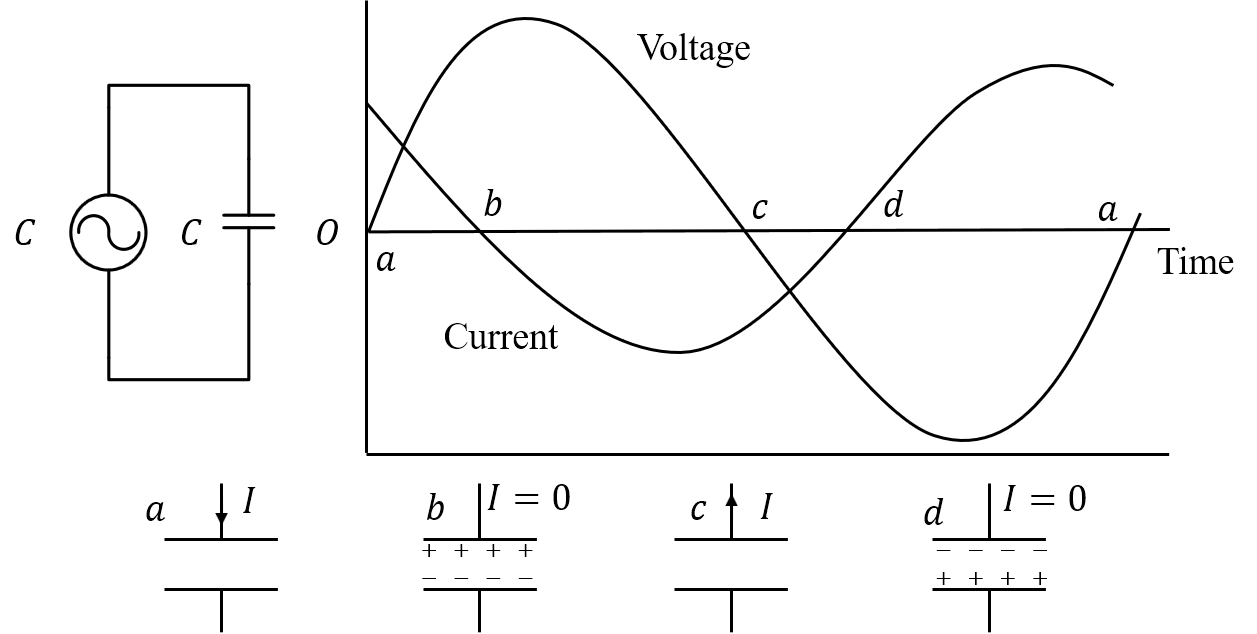
\includegraphics[scale=.75]{ac-circuit-2.png}
\end{figure}
Consider now a circuit which has only a capacitor and an AC power source (such as a wall outlet). A capacitor is a device for storing charging. It turns out that there is a $ 90^\circ $ phase difference between the current and voltage, with the current reaching its peak $ 90^\circ $ (1/4 cycle) before the voltage reaches its peak. Put another way, the current leads the voltage by $ 90^\circ  $ in a purely capacitive circuit.


To understand why this is, we should review some of the relevant equations, including:\\
Relationship between voltage and charge for a capacitor:
\[
    CV = Q
\]
Relationship between current and the flow of change:
\[
    I = \frac{\Delta Q}{\Delta t}
\]
The AC power supply produces an oscillating voltage. We should follow the circuit through one cycle of the voltage to figure out what happens to the current.
\begin{enumerate}[label= Step \arabic*:]
    \item At point $ a $ (see diagram) the voltage is zero and the capacitor is uncharged, Initially, the voltage increases quickly. The voltage across the capacitor matches the power supply voltage, so the current is large to build up charge on the capacitor plates. The closer the voltage gets to its peak, the slower it changes, meaning less current has to flow. When the voltage reaches a peak at point $ b $, the capacitor is fully charged and the current is momentarily zero.
    \item After reaching a peak, the voltage starts dropping. The capacitor must discharge now, so the current reverses direction. When the voltage passes through zero at point $ c $, it's changing quite rapidly; to match this voltage the current must be large and negative.
    \item Between points $ c $ and $ d $, the voltage is negative. Charge builds up again on the capacitor plates, but the polarity is opposite to what it was in step 1. Again the current is negative, and as the voltage reaches its negative peak at point $ d $ the current drops to zero.
    \item After point $ d $, the voltage heads toward zero and the capacitor must discharge. When the voltage reaches zero it's gone through a full cycle so it's back to point $ a $ again to repeat the cycle.
\end{enumerate}
The larger the capacitance of the capacitor, the more charge has to flow to build up a particular voltage on the plates, and the higher the current will be. The higher the frequency of the voltage, the shorter the time available to change the voltage, so the larger the current has to be. The current, then, increases as the capacitance increases and as the frequency increases.


Usually this is thought of in terms of the effective resistance of the capacitor, which is known as the capacitive reactance, measured in ohms. There is an inverse relationship between current and resistance, so the capacitive reactance is inversely proportional to the capacitance and the frequency:\\
A capacitor in an AC circuit exhibits a kind of resistance called capacitive reactance, measured in ohms. This depends on the frequency of the AC voltage, and is given by Capacitive reactance
\[
    X_c = \frac{1}{\omega C}=\frac{1}{2\pi fC}
\]
We can use this like a resistance (because, really, it is a resistance) in an equation of the form $ V = IR $ to get the voltage across the capacitor:
\[V = I X_C\]
Note that $ V $ and $ I $ are generally the r.m.s. values of the voltage and current.
\section{Inductance in an AC circuit}
\begin{figure}[ht]
    \centering
    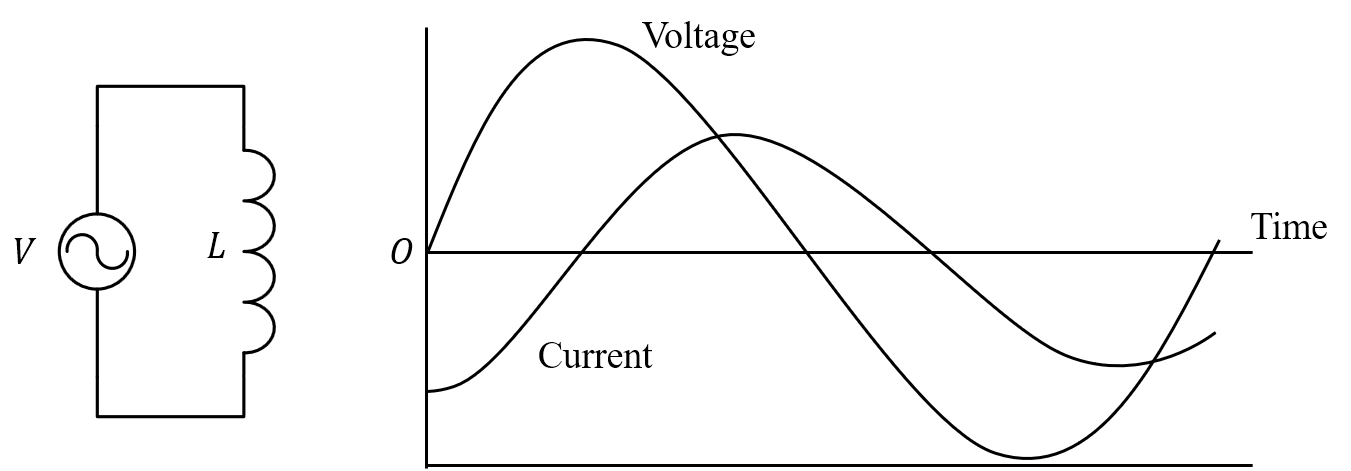
\includegraphics[scale=.75]{ac-circuit-3.png}
\end{figure}
An inductor is simply a coil of wire (often wrapped around a piece of ferromagnet). If we now look at a circuit composed only of an inductor and an AC power source, we will again find that there is a $ 90^\circ $ phase difference between the voltage and the current in the inductor. This time, however, the current lags the voltage by $ 90^\circ $ so it reaches its peak $ 1/4 $ cycle after the voltage peaks.


The reason for this has to do with the law of induction:
\[
    e =-N\frac{\Delta\Phi}{\Delta t} \qquad\text{or}\quad e =-L\frac{\Delta\,I}{\Delta t}
\]
Applying Kirchhoff's loop rule to the circuit above gives:
\[
    V - L\frac{\Delta I}{\Delta t}= 0 \qquad\text{so}\quad V = L\frac{\Delta I}{\Delta t}
\]
As the voltage from the power source increases from zero, the voltage on the inductor matches it. With the capacitor, the voltage came from the charge stored on the capacitor plates (or, equivalently, from the electric field between the plates). With the inductor, the voltage comes from changing the flux through the coil, or, equivalently, changing the current through the coil, which changes the magnetic field in the coil.

To produce a Large positive voltage, a Large increase in current is required. When the voltage passes through zero, the current should stop changing just for an instant. When the voltage is Large and negative, the current should be decreasing quickly. These conditions can all be satisfied by having the current vary like a negative cosine wave, when the voltage follows a sine wave.


How does the current through the inductor depend on the frequency and the inductance? If the frequency is raised, there is less time to change the voltage. If the time interval is reduced, the change in current is also reduced, so the current is lower. The current is also reduced if the inductance is increased.


As with the capacitor, this is usually put in terms of the effective resistance of the inductor. This effective resistance is known as the inductive reactance. This is given by $ X_L = \omega L = 2\pi fL $, where $ L $ is the inductance of the coil (this depends on the geometry of the coil and whether it's got a ferromagnetic core). The unit of inductance is the henry.


As with capacitive reactance, the voltage across the inductor is given by:
\[ V = IX_L\]
\end{document}